% REMEMBER: You must not plagiarise anything in your report. Be extremely careful.

\documentclass{l4proj}

    
%
% put any additional packages here
\usepackage{blindtext}
\usepackage{amsmath}

\begin{document}

%==============================================================================
%% METADATA
\title{Modelling and analysis of dice-based stochastic games}
\author{Lewis Dyer}
\date{}

\maketitle

%==============================================================================
%% ABSTRACT
\begin{abstract}
    This project investigates the use of model checking using PRISM to evaluate the game design of various games of chance involving dice. [RESULTS HERE].
\end{abstract}

%==============================================================================

% EDUCATION REUSE CONSENT FORM
% If you consent to your project being shown to future students for educational purposes
% then insert your name and the date below to  sign the education use form that appears in the front of the document. 
% You must explicitly give consent if you wish to do so.
% If you sign, your project may be included in the Hall of Fame if it scores particularly highly.
%
% Please note that you are under no obligation to sign 
% this declaration, but doing so would help future students.
%
%\def\consentname {My Name} % your full name
%\def\consentdate {20 March 2018} % the date you agree
%
\def\consentname {Lewis Dyer}
\def\consentdate {}
\educationalconsent

\chapter*{Acknowledgements}

I would like to express my gratitude to Dr. Gethin Norman, my project supervisor, for his continual support and guidance throughout the project. I would also like to thank William Kavanagh for offering a number of excellent suggestions throughout the project. Finally, I would like to thank my parents for their encouragement and support throughout what has been a rather eventful year.

%==============================================================================
\tableofcontents

%==============================================================================
%% Notes on formatting
%==============================================================================
% The first page, abstract and table of contents are numbered using Roman numerals and are not
% included in the page count. 
%
% From now on pages are numbered
% using Arabic numerals. Therefore, immediately after the first call to \chapter we need the call
% \pagenumbering{arabic} and this should be called once only in the document. 
%
% Do not alter the bibliography style.
%
% The first Chapter should then be on page 1. You are allowed 40 pages for a 40 credit project and 30 pages for a 
% 20 credit report. This includes everything numbered in Arabic numerals (excluding front matter) up
% to but excluding the appendices and bibliography.
%
% You must not alter text size (it is currently 10pt) or alter margins or spacing.
%
%
%==================================================================================================================================
%
% IMPORTANT
% The chapter headings here are **suggestions**. You don't have to follow this model if
% it doesn't fit your project. Every project should have an introduction and conclusion,
% however. 
%
%==================================================================================================================================

\chapter{Introduction (2 pages?)}

% reset page numbering. Don't remove this!
\pagenumbering{arabic}

Motivate the project. Why is balancing games a challenging problem in the first place? Why is model checking an appropriate tool to examine game design/balance?

\hrule

\Blindtext

\Blindtext

%==================================================================================================================================


\chapter{Background (3 pages)}

Give context on existing work, both in model checking and in automated game design (RMT coursework very helpful for this). Identify a gap in current work (e.g certain types of games that haven't been analysed very much, or discussion on robustness of models). How can I tie this into my project?

Note: don't go into specific details about model types here (MDPs/POMDPs/CSGs) - leave them to later on.

The very key points I need to mention:

\begin{itemize}
    \item Probabilistic model checking
    \item PRISM specifics
    \item Property specification
    \item Stochastic games
    \item Previous work in automated game balancing
    \item Gap in current work (e.g focus on dice/hidden information/weighted dice?)
\end{itemize}

In order to begin formal analysis of a game, we must first formally define a model of a game, along with properties of this game we wish to consider.

\section{Stochastic games}

We first introduce a turn based multiplayer stochastic game (TSG), as described by \cite{kavanagh_balancing_2019}. This model is refined and adapted in each case study to develop a different type of model suited to different types of games.

A turn based multiplayer stochastic game (TSG) is defined as a tuple $(\Pi, S, A, \langle S_i \rangle_{i \in \Pi}, \delta)$ such that:

\begin{itemize}
    \item $\Pi$ is a finite set of players;
    \item $S$ is a finite set of states for a game (for instance, every possible board position in chess);
    \item $A$ is a finite set of actions (such as every possible move in chess, not just those which are possible in the current state);
    \item $\langle S_i \rangle_{i \in \Pi}$ is a partition, such that every state is controlled by exactly one player;
    \item $\delta : S \times A \rightarrow Dist(S)$ is a partial transition function denoting the probability of taking an action in a particular state, where an action $a \in A$ is only available in a state $s \in S$ if $\delta(s, a)$ is defined. $Dist(S)$ denotes the set of discrete probability distributions on $S$.
\end{itemize}

Playing a game is represented as an infinite \emph{path}, denoted as a sequence $\omega = s_0 \xrightarrow{a_0} s1 \xrightarrow{a_1} \dots$ where $\delta(s_k, a_k)(s_{k+1})>0$ for all $k\geq0$, or in other words where each action is possible.

We may also augment this TSG with a set of \emph{reward structures}, which are each comprised of a \emph{state reward function} $\rho : S \rightarrow \mathbb{N}$, associating each state with the value of a reward, and a \emph{state transition function} $\iota : S \times S \rightarrow \mathbb{N}$ which associates each transition with the value of a reward. For instance, in chess, we may define a reward structure where $\iota$ returns $0$ for all transitions, and $\rho$ returns $1$ for all states where a player is in check. Note that the reward values may be continuous (though they may never be negative), but we only consider reward values in $\mathbb{N}$.

\section{Property specification}

When analysing stochastic games, we consider two main types of properties: \emph{probabilistic reachability} properties and \emph{reward-based} properties. We may define properties in terms of \emph{Probabilistic Computation Tree Logic} (PCTL), as defined by \cite{hansson_logic_1994}. These properties are comprised of path quantifiers and temporal operators, though for the purposes of this dissertation we only consider one temporal operator. In particular, the $\mathbf{F}$ operator considers whether a particular proposition \emph{eventually} holds at some state on a given path.

For probabilistic reachability properties, we also include the $\mathbf{P}$ operator, which considers the probability of a particular property holding, including its proposition and any temporal operators, across all possible executions of the TSG. For instance, if we define $\mathtt{game\_over}$ as the proposition that the game is considered to be completed in the current state, the property $\mathbf{P}_{=?} [\mathbf{F}\ \mathtt{game\_over}]$ represents the probability that the game eventually terminates.

For reward-based properties, PRISM defines an extension to PCTL introducing the $\mathbf{R}$ operator, which allows for properties where the value of a reward is taken into account. For the purposes of this dissertation we only consider one type of reward-based property, namely the \emph{reachability reward} property, referring to the expected cumulative value of a reward along a path, until a state satisfying a particular proposition is reached. As an example, using our previous definition of $\mathtt{game\_over}$, the property $\mathbf{R}_{=?} [\mathbf{F}\ \mathtt{game\_over}]$ represents the expected value of a particular reward (such as the number of rounds in a game) before the game is completed.

%==================================================================================================================================

\chapter{Case Study 1: Shut the Box}
\label{cs1}

\section{Game description (1/2 page)}
\label{cs1:stb_description}
Shut the Box is a single player game, where the player aims to cover as many boards as possible through a series of dice rolls. The game starts with a series of \emph{boards}, each numbered sequentially starting from 1, with each board originally uncovered. Each round, the player rolls a set of dice. The player must then cover a set of uncovered boards whose sum is equal to the sum of the dice. For instance, if the player rolls a 1 and a 2, then the player must either cover boards 1 and 2, or cover board 3. The game proceeds in this manner until the player cannot cover a suitable set of uncovered boards. A player's \emph{score} for a round of Shut the Box is defined as the sum of all covered boards.

Throughout the case study, unless otherwise stated, we consider the variant of Shut the Box where there are 12 boards, and the player rolls two six-sided dice each round.

When playing Shut the Box, it soon becomes clear that some configurations of boards are highly desirable, while others are more challenging. For instance, if the only remaining uncovered board is board 10, then the player must roll a 10 in order to continue the game, which occurs with probability $\frac{1}/{12}$. However, if the remaining uncovered boards are boards 1, 2, 3 and 4, then the player may continue with any roll from 2 to 10 inclusive, which occurs with probability $\frac{11}{12}$. Hence, even though each set of uncovered boards currently has the same score, a higher expected score can be obtained starting in the latter configuration. 

Intuitively, this suggests that lower numbered boards are more valuable later in the game, since they increase the set of possible die rolls that a player can roll without ending the game. From this intuition, we develop two potential strategies for playing Shut the Box. The \emph{high-board strategy} is the strategy where the player always elects to cover the highest number board at each stage, while the \emph{low-board strategy} is the converse, where the player always elects to cover the lowest numbered boards at each stage.

When evaluating the effectiveness of these strategies, model checking is a suitable strategy. Since these strategies are deterministic, we may define DTMCs that model Shut the Box under these strategies, define the score of the game as a reward structure, and evaluate the expected score when the game terminates. However, we are also interested in the \emph{optimal} strategy - that is, the strategy which maximises the expected score of Shut the Box. Trying to enumerate and consider every possible strategy would be challenging, both conceptually and computationally. Instead, we consider the case where \emph{no} strategy is defined - in other words, an entirely nondeterministic strategy. In order to achieve this, we consider a generalisation of a DTMC.

\section{Background}
\label{cs1:stb_background}

We start by introducing Markov decision processes (MDPs), which are generalisations of DTMCs allowing for actions to be taken at each state, each leading to different probabilistic transitions between states. We then consider adversaries - resolutions of nondeterministic choice in MDPs - then briefly discuss how optimal adversaries are computed.

\subsection{Markov decision processes}
\label{cs1:mdps}
First, we define an MDP as a modification of a DTMC.

\begin{definition}
\label{cs1:def_mdps}

A Markov decision process (MDP) is a tuple $(S, \bar{s}, \mathbf{Steps}, L)$, where $S$, $\bar{s}$ and $L$ have the same meanings as in Definition \ref{back:dtmc}. $\mathbf{Steps} : S \rightarrow 2^{Act \times Dist(S)}$ is the new transition probability function, where states are mapped to a set of pairs of actions and discrete probability distributions, where $Act$ represents the set of actions the player can take.

\end{definition}

For example, in a game of Shut the Box, $Act$ is the set of possible subsets of boards that the player can cover (such as the action of covering boards 3 and 5 simultaneously). Hence, $\mathbf{Steps}$ maps each state, including the current die value and the current set of uncovered boards, to the set of all possible covering arrangements along with the associated state transition.

Note here that, in general, a state may be associated to more than one action-distribution pair. Indeed, this is where nondeterminism is introduced into the MDP. In order to resolve this nondeterminism, we introduce the concept of adversaries.

\begin{definition}
\label{cs1:adversaries}

Given a \emph{finite} path $\omega = s_0 \rightarrow s_1 \rightarrow \dots \rightarrow s_n$, an adversary is a function $\sigma$ which maps each finite path to an action-distribution pair, more specifically an element of $\mathbf{Steps(s_n)}$.

\end{definition}

A key remark on this definition is that adversaries make decisions depending on the entire execution history up to a state $s_n$, not just the state $s_n$ itself. However, we primarily consider $memoryless adversaries$, where the adversary always picks the same choice in a given state. In particular, this adversary can be viewed as a map from states to action-distribution pairs, as opposed to a map from finite paths to action-distribution pairs. Throughout the remainder of the dissertation, we only consider memoryless adversaries unless stated otherwise.

When an MDP is considered under an adversary, nondeterministic choice is resolved, and a DTMC is obtained. Hence, under a specific adversary, we can apply the model checking techniques introduced in Section \ref{back:prob_mod_check} to evaluate properties of an MDP.

\section{Analysis (3 pages)}

Collect some data, show the results.

\hrule

\Blindtext

\Blindtext

\Blindtext

\section{Evaluation(2 pages)}

The key section - use the results from model checking to answer questions about the game (for instance, to examine the difficulty and/or complexity of a game).

\hrule

\Blindtext

\Blindtext

%==================================================================================================================================

\chapter{Case Study 2 (Liar's Dice)}

In this case study, we introduce Liar's Dice, a dice game utilising hidden information. We introduce partially observable MDPs (known as POMDPs) to represent this hidden information, model a small version of the game using a POMDP, and analyse the susceptibility of Liar's Dice to the snowball effect.

\section{Liar's Dice description}
Liar's Dice is a dice game for multiple players, where each player must be able to bluff and detect opponent's bluffs in order to win. Liar's Dice takes place over a series of rounds, where each player rolls their dice, keeping the values on the dice hidden from other players. A player then makes a \emph{bid}, which is comprised of a face value ono a dice, and the number of dice that show that value. Players then rotate in turn, choosing to either make a higher bid (with either a higher face value, a higher quantity, or both), or challenge the previous bid. If a challenge is made, all dice are revealed. If the bid was correct, the challenging player loses a die. If the bid was incorrect, the bidding player loses a die. The player who lost starts the next round, and play continues until only one player has any remaining dice.

In Liar's Dice, every player starts with the same amount of information, since every player starts with the same number of dice. However, as the game progresses, some players will have more dice than others, changing bidding behaviour, as demonstrated by the following example:

\begin{example}
\label{cs2:hidden_info_example}

Consider the situation presented in Figure \ref{cs2:uneven_information}, where the first player has rolled two 2s while the second player has rolled a 5. The first player can confidently make a bid that there are two 2s, but the second player cannot see enough dice to determine the correctness of this bid. Hence, the second player has three options:

\begin{itemize}

\item If the second player challenges the bid, they will lose a dice, and therefore lose the game.
\item If the second player increases the face value of the bid, then the first player can immediately challenge the bid and win the game, since they know that at most one dice cannot have value 2.
\item If the second player increases the quantity of the bid, to bidding that there are three 2s, the first player can challenge and win with probability $\frac{5}{6}$.

\end{itemize}

As a result, the first player is able to use their increased access to information in order to increase their chances of success.

\end{example}

\begin{figure}[h]
    \centering
    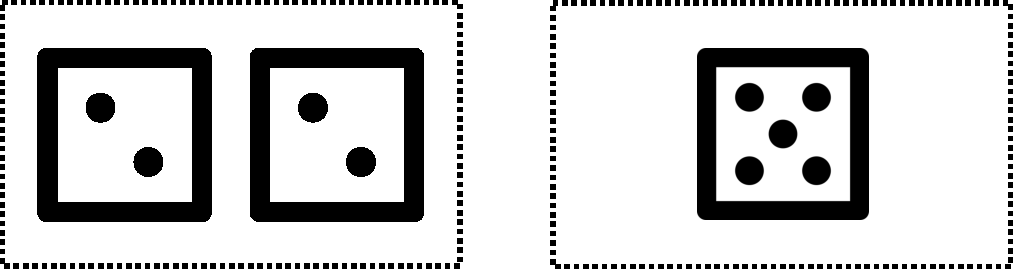
\includegraphics[width=0.7\textwidth]{images/LiarsDice/different_information.pdf}
    \caption{A game of Liar's Dice, where the first player has rolled two 2s while the second player has rolled a 5.}
    \label{cs2:uneven_information}
\end{figure}

This example represents a potential issue with the design of Liar's Dice. Initially we expect that the probability of either player losing a round is even, depending primarily on the strategies the players employ. However, as the game progresses, players with fewer dice are more likely to lose subsequent rounds, making it harder and harder for players to win from behind, a phenomenon known as the \emph{snowball effect} in game design. 

In particular, the snowball effect means that the overall results of games may be decided fairly early on, even if the games are long. This is frustrating for players - the players are still required to play several rounds of a game where the result is already a foregone conclusion. Moreover, with multiple players, this presents an opportunity for one player to be eliminated very early, since the game continues without their involvement.

Our aim when analysing Shut the Box will be to examine to what extent Liar's Dice exhibits the snowball effect, and whether this effect can be mitigated in some way. Firstly, we introduce a variant of MDPs which allows for partial observability, in order to model the hidden information present in Liar's Dice.

\section{Background (1 page)}

A key aspect of Liar's Dice is partial observability, which we now introduce in order to augment our existing MDPs, as described in \cite{norman_verification_2017}.

\begin{definition}
    \label{cs2:def-pomdps}

    A partially observable Markov decision process (or POMDP) is a tuple $\mathcal{P} = (S, \bar{s}, A, \delta, L, \mathcal{O}, obs)$ such that:

    \begin{itemize}
        \item $(S, \bar{s}, A, \delta, L)$ is an MDP, as in Definition \ref{cs1:def_mdps}.
        \item $\mathcal{O}$ is a finite set of \emph{observations}
        \item $obs : S \rightarrow 2^{\mathcal{O}}$ labels each state with a subset of observations.
        \item For any two states $s, s' \in S$, if $obs(s) = obs(s')$ then the available actions at $s$ and $s'$ must be identical. When this occurs, we say that states $s$ and $s'$ are \emph{observationally equivalent}
    \end{itemize}
\end{definition}

The last point in this definition indicates how POMDPs can represent hidden information. Rather than being able to directly access every state, decisions can only be made based on observations. For instance, in many card games, some cards may be visible for a particular player, while others are hidden. In order for two states to be observationally equivalent in a model of this game, we only require that the visible cards are the same in both states, while the hidden cards can range across any permutation of valid cards. If a player could view the full state of the game, they would be able to view the value of hidden cards, which would render most of these games trivial.

Since POMDPs are an extension of an MDP, adversaries for POMDPs are defined in terms of adversaries for the corresponding MDP. However, in order to reflect the added constraints that observations provide, we require that adversaries on observationally equivalent paths are equivalent:

\begin{definition}
\label{cs1:pomdp_strats}

For a POMDP $P$, an adversary of $P$ is a function $\sigma$ mapping all finite paths through the POMDP to a discrete probability distribution over the set of actions. In particular, $\sigma$ is also an adversary of the corresponding MDP. Moreover, for paths $\pi = s_0 \xrightarrow{a_0} s_1 \xrightarrow{a_1} \dots s_n$ and $\pi = s'_0 \xrightarrow{a'_0} s'_1 \xrightarrow{a'_1} \dots s'_n$, if $obs(s_i) = obs(s'_i)$ and $a_i = a'_i$ for all $i \in \mathbb{N}$, then $\sigma(\pi) = \sigma(\pi')$. In other words, $\sigma$ makes the same decisions in observationally equivalent paths.

\end{definition}

This definition references a key difference in optimal adversary generation between MDPs and POMDPs. In MDPs, optimal adversaries are deterministic and memoryless, so in particular adversaries map states to actions. This allows for aforementioned methods such as value iteration to be applied, allowing for efficient computation of optimal values and adversaries attaining these optimal values. By contrast, Madani et al. show in \cite{madani_undecidability_2003} that obtaining optimal values and adversaries, both for reachability properties and reward-based properties, is undecideable. We instead focus on approximate solutions, as discussed in the following section

\subsection{Belief MDPs}

First, we introduce the \emph{belief MDP}. Given a POMDP, we may construct an equivalent MDP, which consists of beliefs of which observationally equivalent state the player is in at any point.

\begin{definition}
    \label{cs2:belief_mdps}

    Given a POMDP $\mathcal{P} = (S, \bar{s}, A, \delta, L, \mathcal{O}, obs)$, as in Definition \ref{cs2:def-pomdps}, the \emph{belief MDP} of $\mathcal{P}$ is given by $\mathcal{B}(\mathcal{P}) = (Dist(S), \delta_{\bar{s}}, A, \delta^\mathcal{B}, L)$. In particular the states of this MDP represent \emph{beliefs} about the state of the player in the corresponding POMDP, and the transition function becomes:

    \begin{equation*}
        \delta^{\mathcal{B}}(b, a)(b') = \sum_{s \in S} b(s) \cdot \left( \sum_{o \in \mathcal{O}, b^{a,o} = b'} \sum_{s' \in S, obs(s')=o} \delta(s, a)(s')\right)
    \end{equation*}

    In particular, $b^{a, o}$ represents the belief reached after performing action $a$ with observation $o$ in belief $b$, calculated using Bayes' Theorem as:

    \begin{equation*}
        b^{a, o}(s') =
        \begin{cases}
            \frac{\sum_{s \in S}\delta(s, a)(s') \cdot b(s)}{\sum_{s \in S} b(s) \cdot \left(\sum_{s'' \in S, obs(s'')=o} \delta(s,a)(s'')\right)} & obs(s') = 0 \\ 0 & \text{otherwise} \\
        \end{cases}
    \end{equation*}

\end{definition}

We also need to modify how state and transition rewards are calculated for a belief MDP.

\begin{definition}
    \label{cs2:belief_rewards}
    Let $\rho$ be a state reward function and $\iota$ be an action reward function for some POMDP $\mathcal{P}$. For the corresponding belief MDP, we set:

    \begin{align*}
        \rho^{\mathcal{B}}(b) &= \sum_{s \in S} rho(s) \cdot b(s) \\
        \iota^{\mathcal{B}}(b, a) &= \sum_{s \in S} \iota(s, a) \cdot b(s) \\ 
    \end{align*}

\end{definition}

In particular, this modification of rewards ensures that reachability and reward-based properties coincide between the POMDP and its corresponding belief MDP.



Describe POMDPs here - what makes them important and useful compared to MDPs? Explain why we add this additional complexity, but also mention trade offs in terms of the sorts of analysis we can perform.


\section{Analysis (3 pages)}

Collect data, show results. Make sure to mention how game trees are constructed to infer results about games based on individual rounds.


\section{Evaluation (2 pages)}

Again, use model checking results to answer questions about Liar's Dice. Discuss potential limitations of analysis that arise from using POMDPs.



%==================================================================================================================================

\chapter{Case Study 3 (26.2)}
\label{ch:cs3}

\section{Game description (1/2 page)}

Again describe the game, come up with some questions to answer about the game. What happens with n players?

\hrule

\blindtext

\blindtext

\blindtext

\section{Background (1 page)}

Introduce CSGs, compare them to MDPs and explain why they're useful for modelling 26.2

\hrule

\Blindtext

\section{Analysis (3 pages)}

Vary different parameters of the game (spaces, number of dice, different strategies...), show results.

\hrule

\Blindtext

\Blindtext

\Blindtext

\section{Evaluation(2 pages)}

Use results to answer questions about 26.2, show the differing behaviour of using different model types.

\hrule

\Blindtext

\Blindtext

%==================================================================================================================================

\chapter{Evaluation (2 pages)} 

Discuss the general process of conducting these case studies. What makes this rigorous research? What could have been improved? Use weighted dice analysis to compare and contrast games. (This is where I could mention experiment automation/preprocessing work to improve replicability)

\Blindtext

\Blindtext


%==================================================================================================================================

\chapter{Conclusion}
\label{conclusion}

The results presented demonstrate that model checking can be an effective tool for answering balance questions about stochastic games. The games presented in these case studies are simple, but even these simple games provide interesting examples of various issues in game design. Shut the Box and 26.2 are both flawed games because optimal strategies are not sufficiently differentiable from simple strategies, while Liar's Dice is flawed because the early rounds of the game have a disproportionate influence on the overall outcome of the game, leading to games which feel artificially long without the later rounds of the game feeling meaningful. Of particular note is the variety of games presented here, with Liar's Dice including hidden information and 26.2 employing simultaneous action selection. This shows the potential of probabilistic model checking for analysing games beyond turn-based perfect information games, which current research primarily focuses on.

While this dissertation has considered numerous different possibilities for analysing games using model checking, a number of further questions are still to be considered.

\begin{itemize}
    \item When generating optimal strategies for games, an important factor in the viability of a strategy is its complexity. As discussed in Section \ref{cs1:eval_stb}, players are unlikely to employ complex strategies if a simpler strategy is similarly effective. However, in general the complexity of a strategy is poorly quantified. Future work in model checking could involve defining a measure for the complexity of an adversary, then penalise strategies which are too complex when computing optimal adversaries. While this will likely lead to less effective strategies, the strategies generated in this manner will be more understandable for human players.
    \item The key bottleneck for further analysis of games is the model size, making full computation infeasible for many realistic games, and improvements in this area would lead to a substantial increase in the viability of model checking for determining game balance. For instance, the game tree construction presented in Section \ref{cs2:state_reduction} could potentially be automated, allowing for subgames to be generated and considered for many types of models.
    \item Another potential avenue for future research is improving the visualisation of generated strategies. In particular, comparing two strategies is challenging, since their visualisations are large and differences in actions are unclear. Improved tool support in this area would be especially useful for designers who are less familiar with formal verification, allowing for optimal strategies to be more easily considered and evaluated.
    \item As briefly mentioned in Section~\ref{cs3:eval_262}, extending probabilistic model checking to partially observable stochastic games would allow for similar techniques to be applied to games where all players have different sets of hidden information, rather than just one player having hidden information, which would allow the techniques presented throughout this dissertation to be employed in a much wider class of games.
\end{itemize}

%==================================================================================================================================
%
% 
%==================================================================================================================================
%  APPENDICES  

\begin{appendices}

\chapter{Appendices}

Typical inclusions in the appendices are:

\begin{itemize}
\item
  Copies of ethics approvals (required if obtained)
\item
  Copies of questionnaires etc. used to gather data from subjects.
\item
  Extensive tables or figures that are too bulky to fit in the main body of
  the report, particularly ones that are repetitive and summarised in the body.

\item Outline of the source code (e.g. directory structure), or other architecture documentation like class diagrams.

\item User manuals, and any guides to starting/running the software.

\end{itemize}

\textbf{Don't include your source code in the appendices}. It will be
submitted separately.

\end{appendices}

%==================================================================================================================================
%   BIBLIOGRAPHY   

% The bibliography style is abbrvnat
% The bibliography always appears last, after the appendices.

\bibliographystyle{abbrvnat}

\bibliography{l4proj}

\end{document}
